\chapter{Аналитический раздел}

В данном разделе проводится анализ предметной области, рассматриваются существующие решения в области электронных библиотек и сервисов для работы с книгами. Формулируются основные требования к проектируемой системе, описываются данные, которые необходимо хранить, а также определяются категории пользователей будущего приложения. На основе проведенного анализа описывается диаграмма вариантов использования и диаграмма сущность-связь проектируемой базы данных.

\section{Анализ предметной области}
Современные библиотеки давно перестали ограничиваться только хранением печатных изданий. В их деятельность входят организация учета большого количества экземпляров книг, газет, журналов и других носителей, ведение информации о читателях и контроль за процессом выдачи и возврата литературы. При традиционном подходе многие операции выполняются вручную: на каждого читателя заводится читательский билет, а библиотекари при резервировании, выдаче и возврате книги делают пометки в соответствующих листах. Такой способ работы трудоемок и подвержен ошибкам. 

Использование информационных систем позволяет автоматизировать эти процессы и существенно повысить удобство как сотрудников, так и посетителей библиотеки, свести к минимуму ошибки при работе с формулярами и ускорить процесс обслуживания. Однако далеко не все библиотеки могут позволить себе дорогостоящее оборудование. Поэтому возникает потребность в разработке доступных решений, которые могут работать на обычных мобильных устройствах без специализированного оборудования.

\section{Анализ существующих решений}
Для анализа были рассмотрены следующие сервисы электронных библиотек: сайт Российской государственной библиотеки для молодежи (РГБМ)~\cite{РГБМ}, сайт библиотеки МГТУ им. Н.Э. Баумана~\cite{МГТУ}, сайт библиотек Москвы~\cite{Moscow}.

Для сравнения решений выделим критерии:
\begin{itemize}
    \item[---] КР1 --- наличие возможности просматривать подробную информацию о книге;
    \item[---] КР2 --- наличие поиска по авторам, ключевым словам и жанрам;
    \item[---] КР3 --- наличие возможности бронировать книги;
    \item[---] КР4 --- наличие возможности добавлять понравившиеся книги в избранное;
    \item[---] КР5 --- наличие возможности вставать в очередь на книгу. 
\end{itemize}

В таблице~\ref{tbl:versus} приводится сравнение существующих решений по приведенным критериям.

\begin{table}[H]
    \begin{center}
        \caption{Сравнение существующих решений}
        \begin{tabular}{|c|c|c|c|c|c|c|}
            \hline
            \textbf{Решение} & \textbf{КР1} & \textbf{КР2} & \textbf{КР3} & \textbf{КР4} & \textbf{КР5}\\
            \hline
            РГБМ & - & + & + & - & - \\
            \hline
            Библиотека МГТУ & + & + & + & + & - \\
            \hline
            Библиотеки Москвы & + & + & + & + & - \\
            \hline
        \end{tabular}
        \label{tbl:versus}
    \end{center}
\end{table}

Из приведенной таблицы видно, что в наибольшей степени заданным критериям соответствуют библиотека МГТУ и библиотеки Москвы. Однако даже они не предоставляют пользователю возможности вставать в очередь на книгу, все экземпляры которой заняты, вынуждая самостоятельно регулярно проверять сайт либо использовать систему уведомлений. 

\section{Формализация задачи}
В рамках курсовой работы необходимо спроектировать базу данных для хранения информации о пользователях, книгах, авторах, издателях, классификаторе, алфавитном указателе, избранных книгах, бронированиях и выдачах, очередях на книгу. Также требуется разработать приложение, предоставляющее графический интерфейс к базе данных с возможностью просмотра, добавления, редактирования и удаления информации из нее. Необходимо рассмотреть несколько пользовательских ролей с разным набором функция и различными правами: гость, читатель, библиотекарь, модератор.

\section{Формализация ролей}
Исходя из предметной области задачи выделим следующие группы пользователей разрабатываемой системы:
\begin{itemize}
    \item[---] гость --- не авторизованный пользователь, который может зарегистрироваться или авторизоваться, а также выполнять поиск по ключевым словам, авторам, жанрам;
    \item[---] читатель --- пользователь, который может выполнять поиск книг, а также добавлять их в избранное, бронировать, вставать в очередь на них. Также читатель должен иметь возможность просматривать свои списки избранного, броней, выдачей и очередей;
    \item[---] библиотекарь --- пользователь, который может изменять статус брони книги, выдавать книги и принимать их обратно;
    \item[---] модератор --- пользователь, который может изменять редактировать информацию о книгах, авторах, издателях, ББК и АПУ. Также модератор может изменить роль другого пользователя в системе.
\end{itemize}

На рисунке~\ref{fig:use-case} приведена Use-case диаграмма выделенных ролей.
\begin{figure}[H]
	\centering
	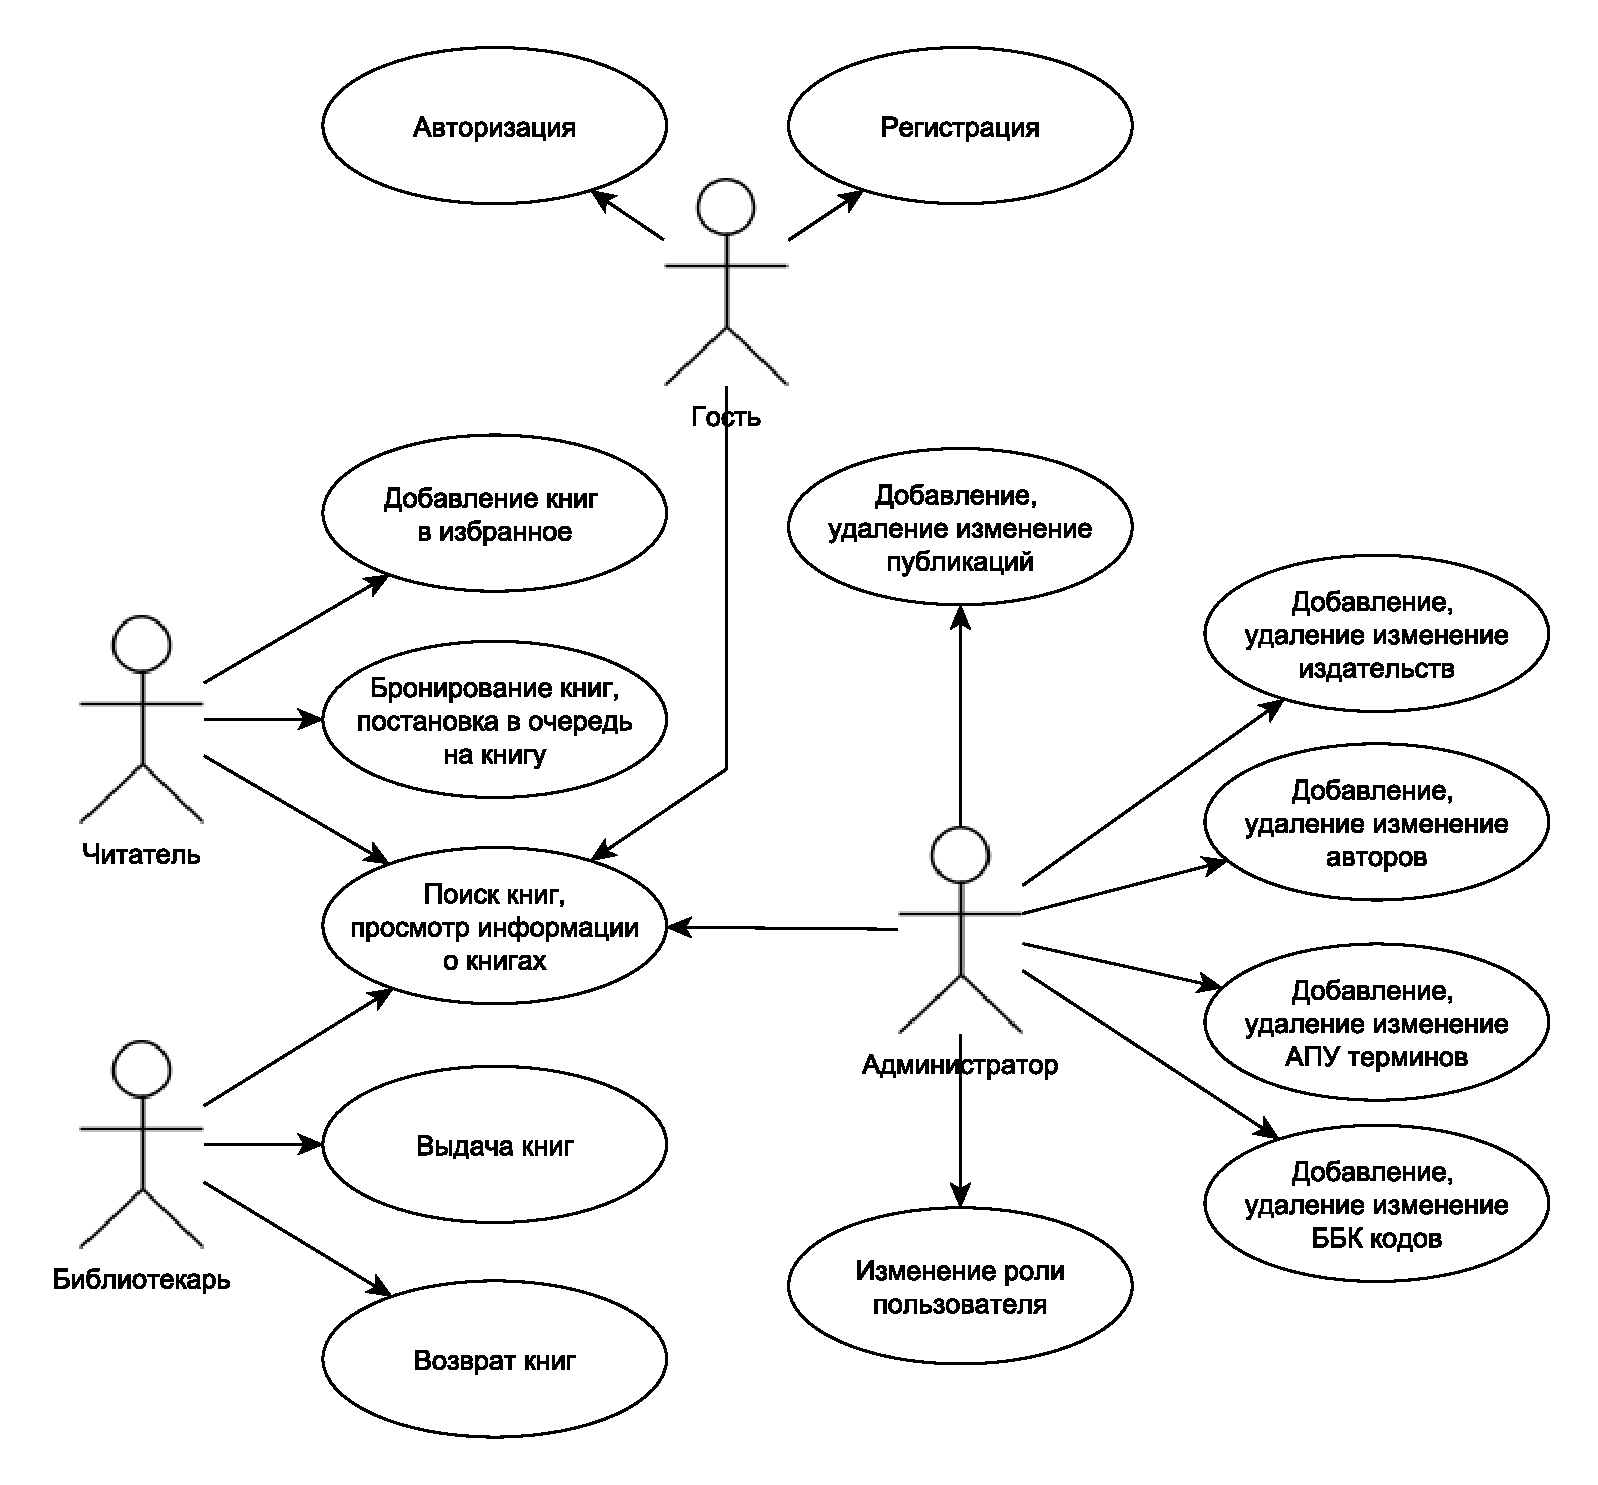
\includegraphics[scale=0.6]{img/use-case.eps}
	\caption{Use-case диаграмма}
	\label{fig:use-case}
\end{figure}

\section{Формализация данных}
Выделим следующие сущности, информация о которых должна быть представлена в базе данных:
\begin{itemize}
    \item[---] пользователь;
    \item[---] книга;
    \item[---] автор;
    \item[---] издатель;
    \item[---] библиотечно-библиографическая классификация (ББК);
    \item[---] алфавитно-предметный указатель (АПУ);
    \item[---] бронь;
    \item[---] выдача;
    \item[---] избранное;
    \item[---] очередь.
\end{itemize}

Какие сведения должна содержать каждая сущность, приведено в таблице~\ref{tbl:entity}
\begin{table}[H]
    \begin{center}
        \caption{Сущности и информация о них}
        \begin{tabular}{|c|p{12cm}|}
            \hline
            \textbf{Сущность} & \textbf{Информация}\\
            \hline
            Пользователь &  Фамилия, имя, отчество, телефон, электронная почта, пароль, роль пользователя в системе\\
            \hline
            Книга & Название, аннотация, автор, издатель, ISBN, формат выпуска, ББК-код, объем, год издания, язык, язык оригинала, количество экземпляров, количество свободных экземпляров\\
            \hline
            Автор & Имя\\
            \hline
            Издатель & Название, описание, телефон, электронная почта\\
            \hline
            ББК & Код, расшифровка\\
            \hline
            АПУ & Термин, соответствующий ББК-код\\
            \hline
            Бронь & Пользователь, книга, дата бронирования, дата отмены бронирования\\
            \hline
            Выдача & Пользователь, книга, дата выдачи, крайний срок возврата, количество продлений\\
            \hline
            Избранное & Пользователь, книга\\
            \hline
            Очередь & Пользователь, книга, дата постановки в очередь\\
            \hline
        \end{tabular}
        \label{tbl:entity}
    \end{center}
\end{table}

На рисунке~\ref{fig:chen} приведена диаграмма сущность-связь в нотации Чена, построенная на основе представленных сведениях об информации, которую должна содержать каждая сущность.
\begin{figure}[H]
	\centering
	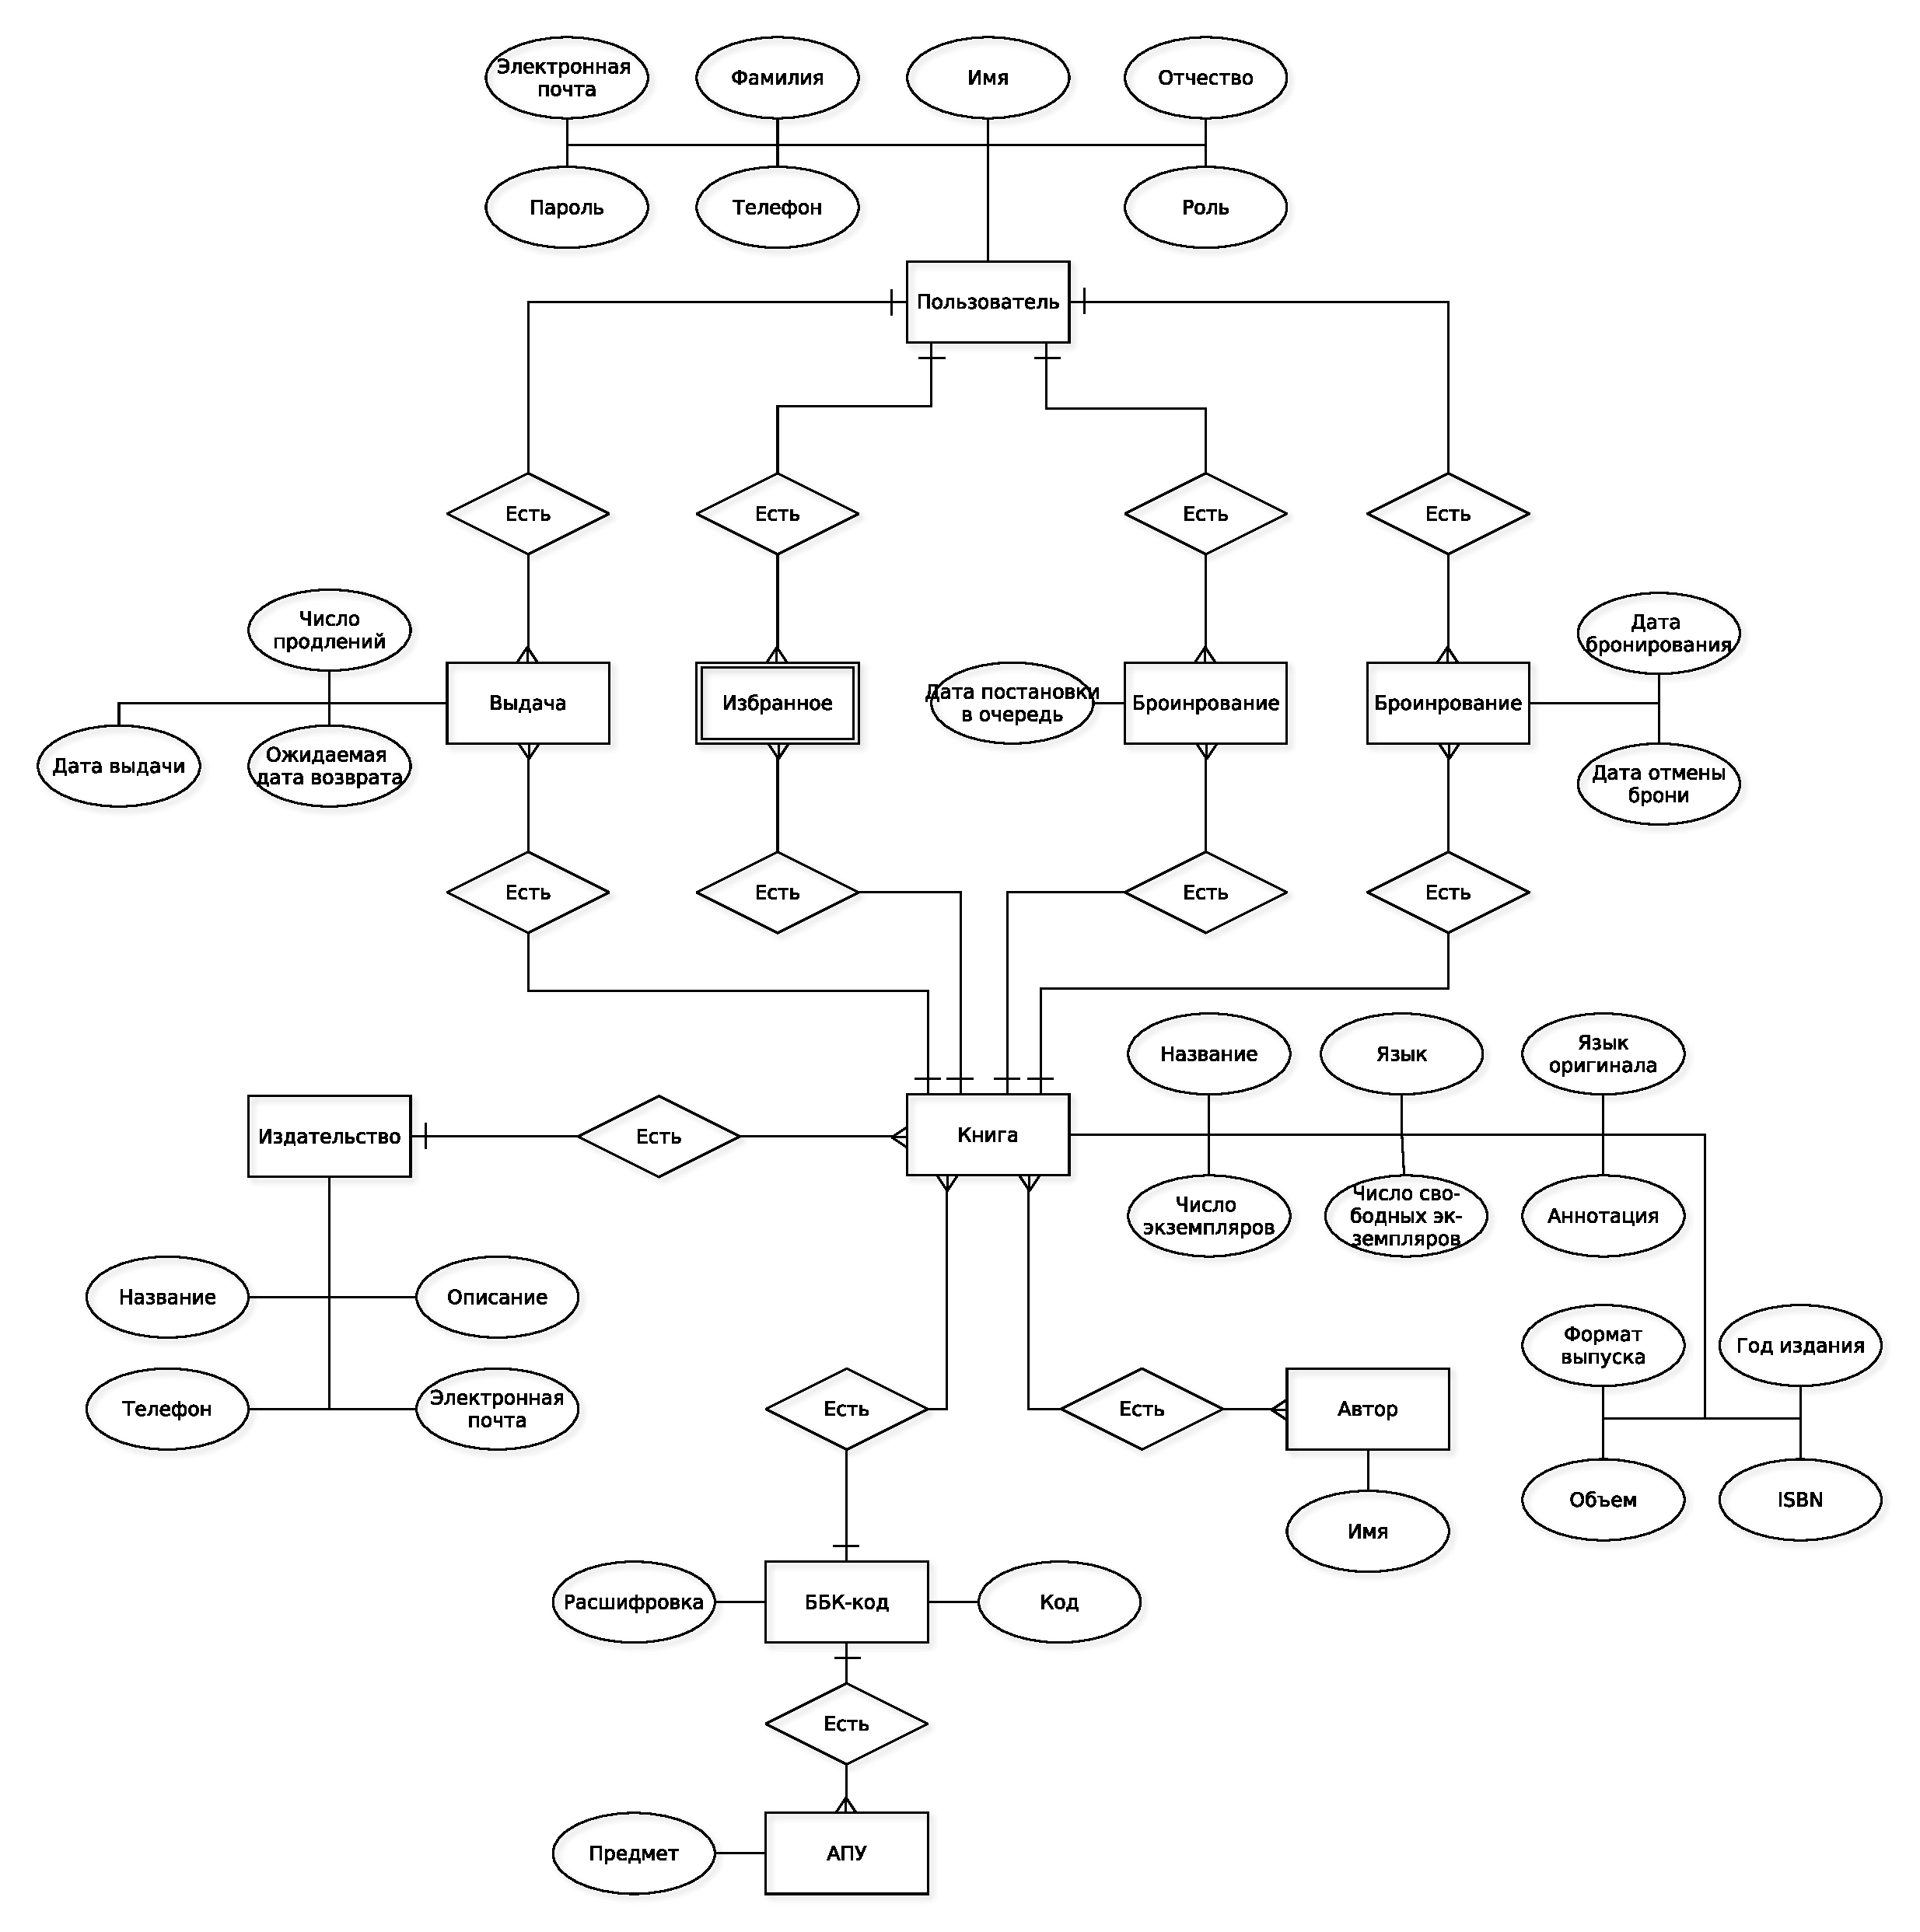
\includegraphics[scale=0.4]{img/ER.eps}
	\caption{Диаграмма сущность-связь в нотации Чена}
	\label{fig:chen}
\end{figure}

\section{Модели баз данных}
База данных --- это совокупность специальным образом организованных данных, хранимых в памяти вычислительной системы и отображающих состояние объектов и их взаимосвязей в рассматриваемой предметной области~\cite{DB}.

Модель представления данных --- представление структуры данных и ограничений целостности, описанных на формальном языке~\cite{Data_model}.

Рассмотрим три основные модели баз данных:

\begin{itemize}
	\item[---] дореляционные;
	\item[---] реляционные;
	\item[---] постреляционные.
\end{itemize}

\subsection{Дореляционные модели данных}
К дореляционным моделям баз данных относят иерархическую и сетевую модели.

В иерархической модели база данных представляется в виде древовидной структуры, состоящей из объектов различных уровней. Между объектами устанавливаются связи типа «предок–потомок»: один объект может включать несколько объектов более низкого уровня, при этом у каждого потомка всегда есть только один предок. Объекты, имеющие одного и того же предка, называются братьями (или близнецами). Основными достоинством иерархической модели данных является простота понимания и использования, к недостатками можно отнести сложности при моделировании связей «многие ко многим» и необходимость дублирования данных.

Для решения проблем иерархической модели была придумана сетевая модель. В ней запись может иметь несколько предков и потомков, благодаря чему уменьшается дублирование данных. Однако сетевые модели обладают сложной структурой, что утяжеляет их разработку и поддержку.

Общим недостатком дореляционных моделей является их зависимость от физической организации данных: изменение структуры часто влечет необходимость переработки прикладной программы.

\subsection{Реляционные модели данных}
Реляционная модель основана на представлении информации в виде таблиц, отношений. Каждая таблица содержит строки и столбцы: строки соответствуют отдельным записям, экземплярам объектов, а столбцы --- их свойствам, атрибутам. Ключевая особенность реляционной модели заключается в том, что данные и связи между ними описываются только с помощью таблиц, а для манипулирования данными используется формальный язык, например SQL. Такая модель обеспечивает высокий уровень абстракции, гибкость при работе с информацией и независимость логического описания данных от способа их физического хранения.

\subsection{Постреляционные модели данных}
Постреляционная модель представляет собой развитие реляционной модели и направлена на снятие ее главного ограничения --- требования атомарности данных в таблицах. В отличие от классического подхода, где каждая ячейка хранит только одно значение, в постреляционной модели допускаются многозначные поля: внутри записи может содержаться набор подзначений, который фактически образует вложенную таблицу.

Такой подход позволяет более естественно отражать сложные структуры данных и упрощает работу с ними. В результате одна постреляционная таблица может совмещать в себе функции нескольких связанных реляционных таблиц, что делает представление информации более наглядным и ускоряет ее обработку.

\textbf{ВЫВОД}

В данном разделе были рассмотрены рассмотрены существующие решения библиотечных сервисов и проведен их анализ по выделенным критериям. Также были формализованы задача, роли пользователей и данные. Были рассмотрены модели баз данных. Была выбрана реляционная модель, так как данные в библиотечной системе легко описываются в виде таблиц, а между таблицами устанавливаются четкие связи.
